\chapter{Social Routing Client Application}
The Social Routing Client Application is a based android application with the objective of representing an user interface of the server functionalities like the
creation, manage and search of a route, for that purpose the behavior of it is based of requests to Web Servers, mostly Social Routing API and Google Maps Platform.
This application has the minimum API level 23 and the target API level is 28, so the platform version is Android 9. Was developed using the Kotlin programming
language, with the goal of the of best code production in the way that was practical and effectual.
The core functionalities of the application require a map to create the routes and to shows it, which was done by using the Google Maps Platform.
All the functionalities of the application are provided from de Social Routing Service, except all that is related to the Google Maps.
All the information is obtained from the server by doing requests to the correspondent endpoint and it is always necessary to send either the token created by
the server or the Google Sign In API tokenId, used on the user registration process. The requests that are related to location retrieval or Map UI require a
specific request to the Google Maps Platform.\\


As an example, the user first experience flow of the application is the following:
        \begin{itemize}
                \item The user provides his google account credentials to authenticate with the application, which in its turn makes a request to the backend server.
                \item The user will be redirected to a navigation screen that contains a route search bar and a left panel menu with buttons to redirect to the screens of user profile and route creation.
                \item After the user searches routes using a location, happens a redirection to a new screen in which contains a list of found routes.
                \item Once a route is chosen and pressed upon, a new activity with a map is shown, where the route is represented and with a button to start Live Tracking.
                \item By choosing to start Live Tracking the user location is now showed as well as a path to reach the beginning of the chosen route.
                \item If the user wants to see the his profile he may go back until the navigation screen and click in the left panel and then in the User Profile button.
                \item In the user profile the user information (user rating, name and routes created) is shown.
                \item For creating a route, a button press in the bar menu is required.
                \item This action takes the user to a new screen that shows the map, a button to finish and a form, asking the location of the route that will be created.
                \item The user must then insert the location on which the map will zoom in.
                \item A click in the map will add the pressed location point to the route being created. If something wrong occurs the user can delete the last point of the route clicking the button on the top of the screen.
                \item A button continue always in the screen until be clicked to finish the first part of the route creation, which pops up all the places of interest near of the route created.
                \item When finished the user click in the button finish to fill the final form that contains the name, description and category of the route and that is contained in the RouteCreationMetadataActivity.
                \item After the form is filled the user is redirect again to the route representation of the route that was just created.
        \end{itemize}

\begin{figure}[h]            
        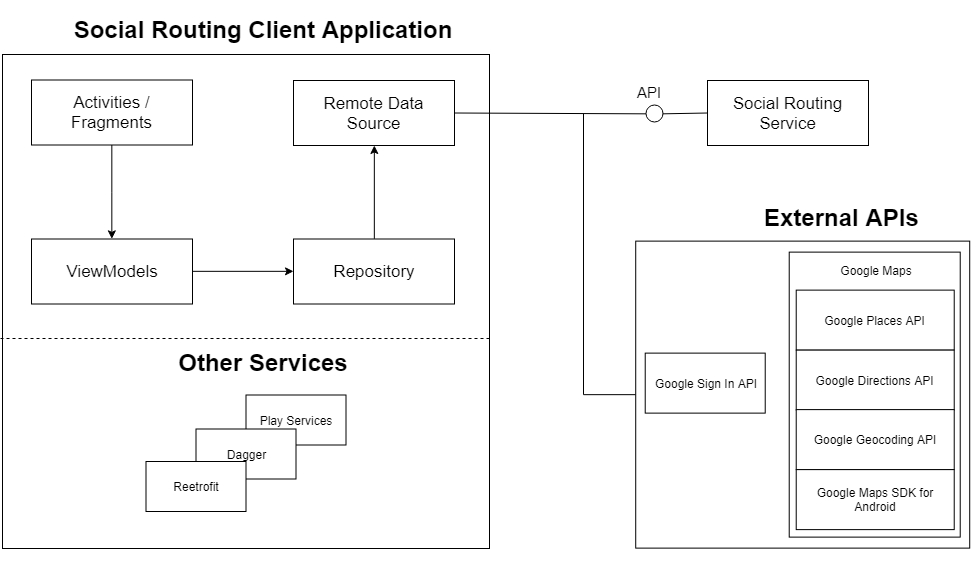
\includegraphics[width=\textwidth]{images/project-structure/social-routing-client-application-structure.PNG}
        \caption{Social Routing Client architecture.}
        \label{fig:clientarchitecture}
\end{figure}

The Social Routing Client Application is composed by four major components, each with it's own compromise and objective.
The Activities\cite{activities} and Fragments\cite{fragments} to represent the User Interface (UI) where the user can interact with the application, the 
View Models\cite{viewmodel} to store and manage UI related data, a Repository that handles data operations and knows where to retrieve data from and a 
Remote Data Source to communicate with external components, for instance the Social Routing API, the Google Sign In API or Google Maps Platform. 
This logic is represented in the figure \ref{fig:clientarchitecture}.
Internal Services were used to complement the application, to do some difficult work for us. The internal providers used to make everything work properly were:
\begin{itemize}
        \item Retrofit: with the intention of making HTTP requests to web servers and obtain data if necessary.
        \item Dagger: objective of injection of needed dependencies in development context.
        \item Play Services: principal provider of the google maps via intent to all the activities that create or are visible.
        \item Google Sign In: used to authenticate in the Google Account, provided also from Intent.
\end{itemize}   

\section{Remote Data Source}
Module that has the objective of communicating with external APIs which it does by executing requests to either the Social Routing API, the Google Maps Platform or the Google Sign In API. 
The Component knows the structure of the HTTP request to the endpoints, like the parameters and meta-data necessary to obtain the required Response. After the request is done, the webservers\cite{webserver} 
provide the response in the JSON\cite{jsonwebsite} format, however the response is deserialized using the library Jackson\cite{jackson}, to convert it to Object. 
So was defined all the input model objects, to automatically deserialize the response to object.\\

\section{Repository}
The Repository handles data operations, knows where to get the data from
and what API calls to make when the data is updated. A repository can be
considered a mediator between different data sources, such as web services. \\
The application has repositories specified to the Social Routing API and another to Google Maps Platform, which contains
multiple APIs. Each one as correspondent Web Service that uses the
framework Retrofit\cite{retrofit}, used to make a synchronous or asynchronous HTTP request to the remote webserver. The Repository obtains the data
from the web server and can only have two possible request status: Failure or Success. It returns the data contained in a LiveData\cite{livedata} because when the data 
updates can then be observable. \\
The Repository specific to our API (Social Routing API) discovers all the endpoints by doing a request to the root endpoint, 
depending on the objective and the functionality, like the endpoints to sign in, to get user info, routes, create a route, get all categories, update a route, amongst others. \\
On the other hand the other repository is used to make request to the Google Webserver (Google Maps Platform) about the geocode\cite{geocode} of a location, the directions to a 
coordinate in the map and the places of a given area. 

\section{View Models}
Component used when the UI experiences a change. The View Model calls
other components to load the data, and it can forward user requests to
modify the data however it doesn't know about UI components, 
it is completely separated from them. \\
This component has a simple implementation, the application contains three View Models one for the Routes information (get, creation, update, search), 
to the User (get, update) and another to the Google Maps Platform (information of a location, places, directions). It uses the repository to obtain the data and 
then return it in the shape of Livedata.

\section{Activities/Fragments}
The only concern of this component is to provide a way for the user to interact with the application and with the view.
All activities extend a BaseActivity that has a global behavior such as when the data is changed, is necessary to update the view and to show some view components 
like a toast\cite{toasts}, progress bar\cite{progressBar} or even start another activity, to be more noticeable to the user what is happening on the application.\\

Each Activity has its own :
\begin{itemize}
        \item Design: defined by one or more layouts that contains buttons, images, input text, fragments (for instance the map fragment provided by Google), 
        with which the user can interact and make actions.
        \item Behavior: when the data changes the view needs to be updated, behavior this, that is defined with either a success or error, using the ViewModel.
\end{itemize}

\subsection{BaseActivity}
\begin{itemize}
        \item Design: No layout.
        \item Behavior: Is an abstract implementation of an Activity that contains generic behavior to view components and knows how to handle changes in the Livedata from View Model, 
        to all the Activities that implement it.
\end{itemize}

\subsection{LoginActivity}
\begin{itemize}
        \item Design: Login Activity Layout.\cite{loginactivitylayout}
        \item Behavior: Where the Authentication(\ref{authentication}) happens, using the google account credentials the user can login/authenticate in the server side and a
request to the Root endpoint of the Social Routing API is done.
\end{itemize}

\subsection{NavigationActivity}
\begin{itemize}
        \item Design: Navigation Activity Layout.\cite{navigationactivitylayout}
        \item Behavior: The client can navigate through the application functionalities with this activity. This layout contains a text box to input the location, to search for the best 
route possible, a list that shows the closest routes to the user current location, doing a request to the Social Routing Service with the default filters like all categories,
a route with short duration and finally a panel that contains buttons to go to other activities, like RouteCreationActivity(\ref{routecreationactivity}) and 
UserProfileActivity(\ref{userprofileactivity}).
\end{itemize}

\subsection{RouteCreationActivity} \label{routecreationactivity}
\begin{itemize}
        \item Design: Route Creation Activity Layout.\cite{routecreationactivitylayout}
        \item Behavior: A core functionality of the Social Routing Client Application is in this activity, because is where the user can create a route and it's corresponding metadata.
        Initially a Fragment is obtained asynchronously, provided by the Google Play Service\cite{googleplayservices}, that represents the Google Maps\cite{googlemaps}. Right after the map is the RouteDetailsActivity
        a form pops up asking for the desired location of the route, to be created. After the user inputs the location name, a request is made to Geocoding API\cite{geocodingapi} from google to obtain 
        the geocoordinates to do a zoom in the map. Then the user can click in the map to select the route points in order to create the path to be saved. When the route path is 
        finished, the user must click in the button continue to proceed to the Places of interest, that is, a request is made to the Google Places API\cite{googleplacesapi} to obtain the Places Of interest
        near the route points (in a range of one hundred meters) that can be added as metadata of the route. To conclude, calculations are made to discover if the route is circular or not, by doing a radius circle from
        the first route point selected in the map and if the last point selected is inside the radius, it means that the route is circular and will be represented with no initial point, otherwise 
        the route is not circular and could be ordered, if selected. 
\end{itemize}
\newpage
\subsection{RouteCreationMetadataActivity} \label{routecreationmetadataactivity}
\begin{itemize}
        \item Design: Route Creation Metadata Layout.\cite{routecreationametadatactivitylayout}
        \item Behavior: The objective of this activity is the termination of the route creation. It receives the route information that was obtained from the previous activity (RouteCreationActivity[\ref{routecreationactivity}])
        via Intent \cite{intent}. The user is then required to fill some input fields about the route like the name, description, categories, if it's ordered or not, duration and image to fully create the route and make a POST 
        request to the Social Routing Service to be created. If the request succeeds, the route representation is shown in the RouteRepresentationActivity(\ref{routerepresentationactivity}).
\end{itemize}

\subsection{RouteDetailsActivity}
\begin{itemize}
        \item Design: Route Details Activity Layout.\cite{routedetailsactivitylayout}
        \item Behavior: Activity to represent some metadata of the route like the name, description, categories, duration and image that are obtained via Intent and are represented to the 
        layout.
\end{itemize}

\subsection{RouteRepresentationActivity} \label{routerepresentationactivity}
\begin{itemize}
        \item Design: Route Representation Activity Layout.\cite{routerepresentationactivitylayout}
        \item Behavior: Through Intent the route URL\cite{url} is sent  to this activity, to do a request to Social Routing Service and obtain all the route detailed information. The Google Maps
        is initialized and the route path is shown to the user with blue markers and lines that are drawn in the map and the places of interest with red markers. If the route is circular the first and last point are unified by a line.
\end{itemize}

\subsection{RouteSearchActivity}
\begin{itemize}
        \item Design: Route Search Activity Layout.\cite{routesearchactivitylayout}
        \item Behavior: The search functionality is done with specific filters (categories, duration and location) and it is done in this activity, by passing the correspondent parameters to it
        and making a request to the Social Routing API. If successful the results are shown in a list.
\end{itemize}

\subsection{UserProfileActivity} \label{userprofileactivity}
\begin{itemize}
        \item Design: User Profile Activity Layout.\cite{userprofilectivitylayout}
        \item Behavior: Previously a request was done to the root endpoint to obtain the URLs of the API and also retrieve the user profile URL of the user authenticated that is used to make 
a request to obtain all the information about it.
\end{itemize}

\newpage

\section{External Services}
For the realization of the Social Routing Client Application to be possible, external libraries were used, like the Google Places API, Google directions API and
Google geocoding API, to obtain the information about locations, places and even just to the geographic coordinates of a location. All these services were used to support
the route creation for instance, because all the route information and meta-data can only be obtained via external providers. However some of this services were
also required by the search for a route functionality, because the user input is a location name but the Social Routing Service API requires a place identifier to make a valid request from.
Because of that, to obtain that information, the Google geocoding API was used. It retrieves the information of the place, like the Identifier. Thus the external services are
a core component of this application because without them it would not be materialized.

\section{Authentication} \label{authentication}
For the Social Routing Client Application to be able to make requests to the Social Routing Service, it needs to obtain valid authentication first, except when requesting the API root endpoint.
Thus first things first, the user needs to authenticate and for that is provided a Google Sign In button that when clicked will redirect the user to an Intent provided
by Google Play Services that permits the login/registration with the user's Google account. After all that Google processing, the user is redirected again to the application with
Google Account information like name, email and id token. The user name and email are just representative in the view components, however the id token provided is used
to authenticate in the Social Routing Service, by doing a POST request where the body contains the id token. When the response is obtained it only has two
possibilities: success or error. If all goes well,  an Authentication object is obtained, which contains the access token, the refresh token and the user URL,
on the other hand, if the result is invalid then it is not possible to make requests to the service. It is only possible to make requests to the Social Routing Service when the id token is valid. The access token is sent in all
the requests done to the Social Routing Service to obtain or send information, however that access token expires. When this happens, another POST request is sent
to refresh the token, by sending the refresh token in the request body provided initially.